\section{Results and Analysis}
\label{analysis}

We analyze Mini-MAC for performance and authentication strength. 
Mini-MAC must be able to authenticate messages 
without compromising the performance of the real-time, safety-critical systems.

\subsection{Performance}
\label{performance}

Tables~\ref{tab-traffic}--\ref{tab-time} and Figures~\ref{fig-execution}--\ref{fig-code}
show the message traffic, execution time, code size, and RAM usage of our unoptimized implementations
of Mini-MAC and their underlying HMACs.  Time and space are dominated by the HMAC computation.

%Throughout, ``B''~denotes bytes, ``b''~denotes bits, and ``ms''~denotes milliseconds.

Table~\ref{tab-traffic} shows that Mini-MAC adds no additional bus traffic.
By contrast, HMAC-MD5 adds 128~bits (two CAN frames) per authentication,
due to the 128-bit tag.  Similarly, the pairwise-keyed Lin-MAC generates
two additional CAN frames per recipient ECU in each group communication.

Table~\ref{tab-time} shows the mean observed execution time
and standard deviation for each of our implementations of Mini-MAC.
Using MD5 is much faster than using SHA-1 or SHA-2.  As shown in Table~\ref{tab-overhead},
the overhead in time to compute Mini-MAC beyond HMAC is very little (approximately 0.38--0.68~ms).
Similarly, Figure~\ref{fig-execution} shows the mean observed execution times for Mini-MAC measured
in number of cycles on a 32~kHz clock.

Importantly, Table~\ref{tab-time} shows that only our 
MD5 implementation of Mini-MAC runs fast enough to satisfy our
requirement of authenticating at least 40 messages per second (approximately
25~ms between messages).   
While highly optimized code will likely run faster, on the
basis of our timing measurements, we recommend implementing Mini-MAC using MD5.

Figure~\ref{fig-ram} shows the RAM usage for our implementations of Mini-MAC.
As shown in Table~\ref{tab-overhead}, the overhead in RAM usage to compute Mini-MAC
beyond HMAC is very low (5~bytes).

Figure~\ref{fig-code} shows the code size of our Mini-MAC implementations.
As shown in Table~\ref{tab-overhead}, the additional code size for Mini-MAC beyond
HMAC is very small (approximately 800~bytes).
	
\subsection{Authentication Strength}
\label{security}

Mini-MAC detects spoofed messages by using a keyed HMAC.  It detects replay attacks
by incorporating a counter and recent message history into the HMAC input.  Using message
history also complicates a transient attacker who may be unable to observe a sufficient
number of recent messages.  

	\fontfamily{ptm}\selectfont
	\begin{figure}
		\centering
		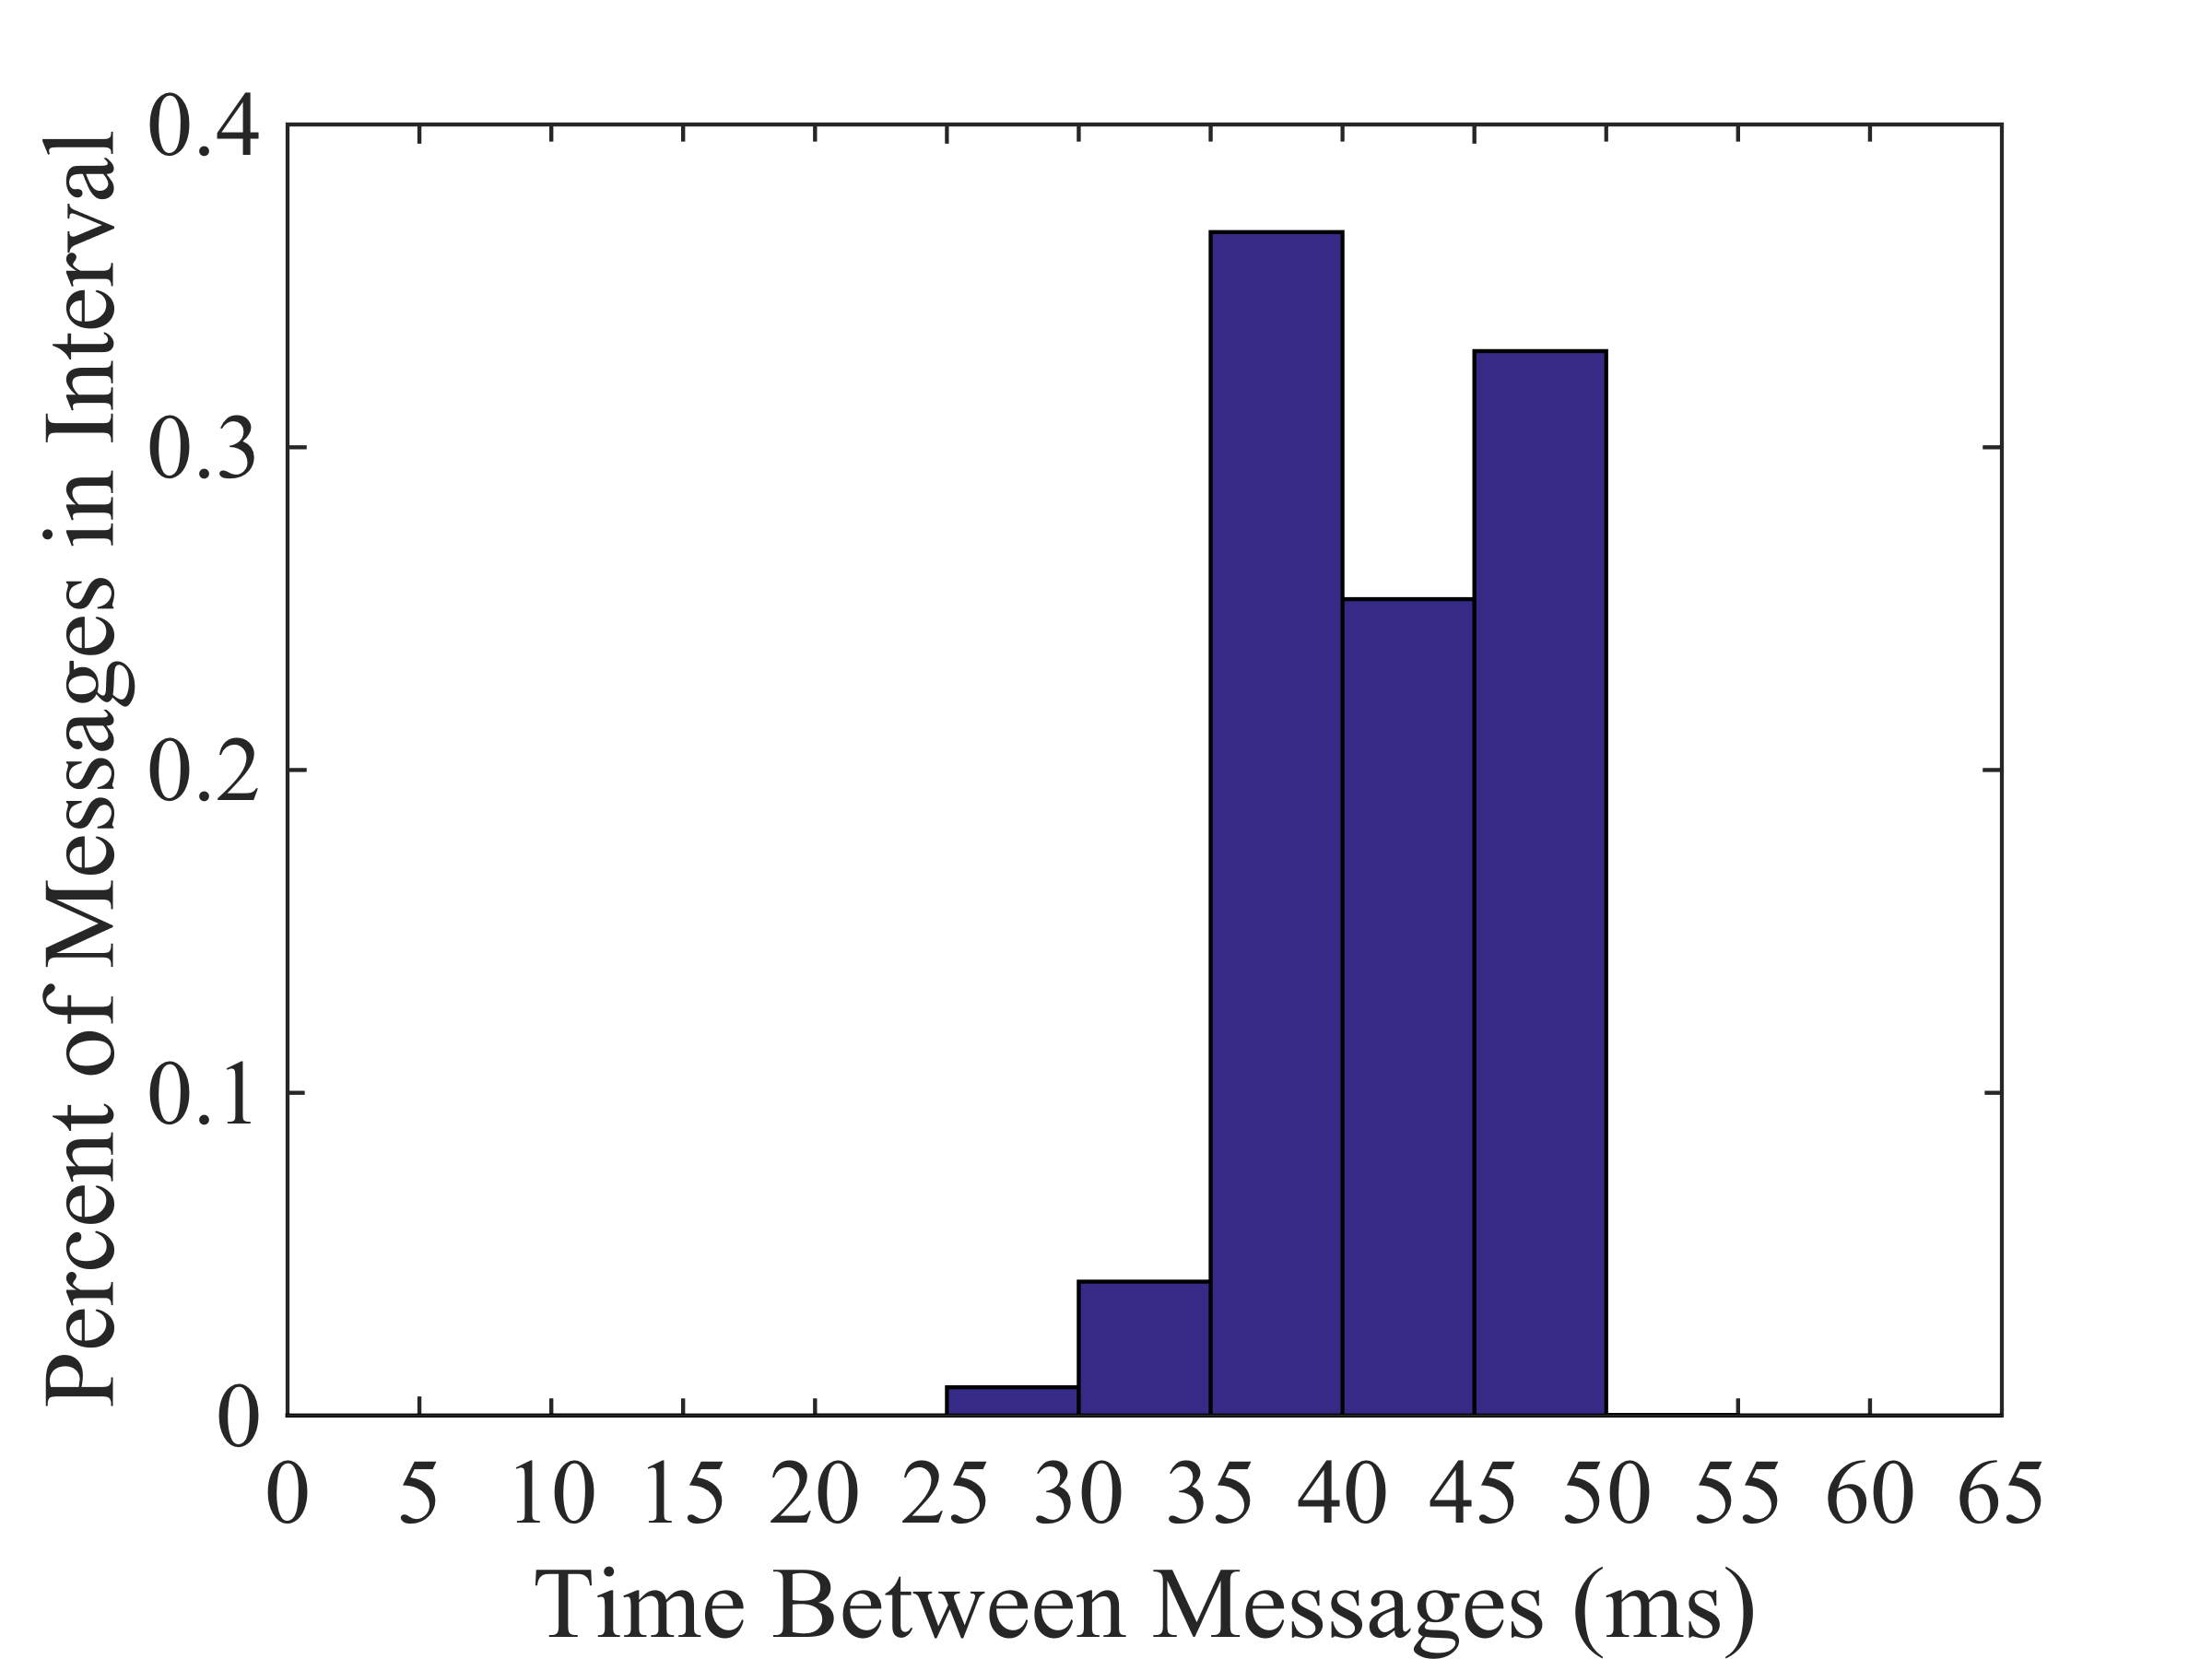
\includegraphics[width=\columnwidth]{figures/relative_histogram.png}
		\caption{{\fontfamily{ptm}\selectfont Histogram 
		of message interarrival times observed by the authors from 
		15,768 messages on a 2010 Toyota Prius. }}
		\label{fig-msgdelay}
	\end{figure}

\begin{table*}	
	\centering
	
	\caption{Probability and expected time for a spoofed message to be accepted by an ECU for various tag lengths
	for two attack scenarios.  In random guessing, the adversary guesses a tag.
	In the hypothetical collision search, the adversary seeks a Mini-MAC collision.
	Probability denotes the probability of success for one trial.
	Expected time denotes the expected time for the cumulative success probability to be~0.5.
	All calculations assume the adversary injects 40 forged messages per second.}
	
	\label{tab-taglength}
	\vspace{8pt}
	\begin{tabular}{c|rrl|rl}%
	{\bf Tag Length (bits)} & {\bf Random Guessing} &&& {\bf Collision Search} & \\
	& {\bf Probability} & {\bf Time} & & {\bf Time} & \\\hline
	8  & 0.0039 & 3.20 & sec & 0.40 & sec \\
	16 & 1.53\text{\sc{e}-}05 & 13.65 & min & 6.40 & sec \\
	24 & 5.96\text{\sc{e}-}08 & 58.25 & hour & 1.70 & min \\
	32 & 2.33\text{\sc{e}-}10 & 621.38 & day & 27.30 & min \\
	40 & 9.09\text{\sc{e}-}13 & 435.82 & year & 7.28 & hour \\
	48 & 3.55\text{\sc{e}-}15 & 111,568.9 & year & 4.85 & day \\
	\end{tabular}
	\end{table*}

The 128-bit keys are sufficiently long to withstand 
exhaustive key-search attacks.  The 64-bit counter is sufficient to prevent counter
rollover within the lifetime of the car.

%With $\lambda = \hbox{72,000}$, the adversary must learn over 30~minutes of recent
%message history.

A security-enhancing feature of the CAN bus is, ironically, its slow speed of at most
approximately 40 messages per second.  Figure~\ref{fig-msgdelay} shows a histogram of
message arrival times that we collected from a 2010 Toyota Prius.
The slow speed of the CAN bus limits the rate at which an attacker can
inject messages into the bus.

Another defensive feature is that there is no simple fast way for an adversary to
test if a candidate tag is valid.   The only way we are aware of is to inject a message into the bus
and observe if the receiving ECU accepted the message.

Limitations imposed by Mini-MAC include its use of group keys and truncated HMAC tags.  
Using group keys means that a single compromised ECU learns all of the keys
to which groups it belongs.  We consider this limitation an acceptable design tradeoff
given that Mini-MAC does not increase bus utilization and the compromise of any critical
ECU is a devastating security failure.

One potential attack is for the adversary to inject messages into the bus with the hopes
of trying a tag that verifies correctly.  We shall call this attack the ``trial injection attack.''
A downside of this attack is that it would be easy to detect such an attack involving
many messages.

Table~\ref{tab-taglength} lists for various tag lengths~$L$
two reference times that are useful in assessing the effectiveness of this and other hypothetical attacks.
The ``random guessing'' columns refer to the strategy of randomly guessing tags.
Probability denotes the probability that one guess will be accepted as valid; this probability
is $1/2^{L}$, where $L$ is the tag length.
Expected time denotes the expected time for the cumulative success probability to be~0.5,
assuming the adversary is limited to trying 40 tags per second.
This value is the expected time for a straight-forward 
implementation of a trial injection attack to succeed.  

The ``collision search'' column refers to an optimistic hypothetical attack whose success is based on
finding a Mini-MAC collision,\footnote{A collision is any pair of 
different inputs that produces the same output.}
exploiting the Birthday Paradox.  
We do not see how an adversary could mount such an attack;
we include this column simply as a conservative reference.

For example, with a four-byte tag, the expected time for a straight-forward 
message injection attack to succeed is over 621~days.  

Another potential attack is to observe bus traffic with the hopes of finding statistical
regularities that would significantly improve the chances of success of the aforementioned attack.
We conjecture that this attempt is unlikely to yield significant advantage, given the
strong properties of HMAC and some
desirable (albeit imperfect) characteristics of the component hash functions.

Given that the CAN bus does not authenticate messages, we conclude that Mini-MAC
meaningfully raises the bar of vehicular security.


	
